%&-job-name=newfilenameialwayswanted
\documentclass[
a4paper, % Stock and paper size.
12pt, % Type size.
article,
% oneside, 
onecolumn, % Only one column of text on a page.
% openright, % Each chapter will start on a recto page.
% openleft, % Each chapter will start on a verso page.
openany, % A chapter may start on either a recto or verso page.
]{memoir}
\synctex=1
\maxtocdepth{subsection}
\setsecnumdepth{subsection}
\counterwithout{section}{chapter}
%%% PACKAGES 
%%%------------------------------------------------------------------------------
\usepackage[utf8]{inputenc} % If utf8 encoding
% \usepackage[lantin1]{inputenc} % If not utf8 encoding, then this is probably the way to go
\usepackage[T1]{fontenc}    %
\usepackage[english,russian]{babel} % English please


%%% Figures and colors
\usepackage[usenames,dvipsnames,svgnames,table,rgb]{xcolor}
\usepackage{tikz} % Figures. Following colors are predefined: red, green, blue, cyan, magenta, yellow, black, gray, darkgray, lightgray, brown, lime, olive, orange, pink, purple, teal, violet and white.

% Defining a new coordinate system for the page:
%
% --------------------------
% |(-1,1)    (0,1)    (1,1)|
% |                        |
% |(-1,0)    (0,0)    (1,0)|
% |                        |
% |(-1,-1)   (0,-1)  (1,-1)|
% --------------------------
\makeatletter
\def\parsecomma#1,#2\endparsecomma{\def\page@x{#1}\def\page@y{#2}}
\tikzdeclarecoordinatesystem{page}{
    \parsecomma#1\endparsecomma
    \pgfpointanchor{current page}{north east}
    % Save the upper right corner
    \pgf@xc=\pgf@x%
    \pgf@yc=\pgf@y%
    % save the lower left corner
    \pgfpointanchor{current page}{south west}
    \pgf@xb=\pgf@x%
    \pgf@yb=\pgf@y%
    % Transform to the correct placement
    \pgfmathparse{(\pgf@xc-\pgf@xb)/2.*\page@x+(\pgf@xc+\pgf@xb)/2.}
    \expandafter\pgf@x\expandafter=\pgfmathresult pt
    \pgfmathparse{(\pgf@yc-\pgf@yb)/2.*\page@y+(\pgf@yc+\pgf@yb)/2.}
    \expandafter\pgf@y\expandafter=\pgfmathresult pt
}
\makeatother

\usepackage{graphicx}  % Include figures
\usepackage{wrapfig}
\graphicspath{{img/}{../img/}} 


%%% INTERNAL HYPERLINKS
%%%-------------------------------------------------------------------------------

\usepackage{hyperref}   % Internal hyperlinks
\newcommand{\linkcolor}{blue}
\newcommand{\citecolor}{blue}
\newcommand{\filecolor}{magenta}
\newcommand{\urlcolor}{NavyBlue}
\hypersetup{				% Гиперссылки
    pdfborder={0 0 0},      % No borders around internal hyperlinks
	unicode=true,           % русские буквы в раздела PDF\\
	pdfstartview=FitH,
	colorlinks=true,  % false: ссылки в рамках; true: цветные ссылки
	linkcolor=\linkcolor,         % внутренние ссылки
	citecolor=\citecolor,        % на библиографию
	filecolor=\filecolor,      % на файлы
	urlcolor=\urlcolor,      % на URL
    linkbordercolor=\linkcolor,  % hyperlink border will be red 
    pdftitle={Yoga Veera Kit},
    pdfpagemode=FullScreen,
    pdfauthor={I am the Author} % author
}

\let\oldhref\href
\renewcommand{\href}[2]{\oldhref{#1}{\underline{#2}}}

   
\graphicspath{{img/}{../img/}{../FreqImg/}}


%%% PAGE LAYOUT 
%%%------------------------------------------------------------------------------

\setlrmarginsandblock{0.15\paperwidth}{*}{1} % Left and right margin
\setulmarginsandblock{0.10\paperwidth}{*}{1}  % Upper and lower margin
\checkandfixthelayout
%%% indenting
\setlength{\parindent}{0em}
\setlength{\parskip}{0.5em}
\begin{document}
\begin{center}
    \Huge \textbf{Русский гайд}
\end{center}
\tableofcontents

\tikz[remember picture,overlay] \node[opacity=0.9,inner sep=0pt] at (page cs:0.8,0.8){
\includegraphics[width=0.1\paperwidth]{IshaLogo}};

\section{YouTube Videos Translation Process}

\subsection{\ldots}
\ldots
\subsection{Создание аудио трека}
Подробнее должен рассказать Эльдар.
\subsection{Создание финального видео}
\subsubsection{AirTable}
Эльдар после создания аудио трека отмечает ответственного за этот этап в AirTable. В последнем можно будет найти ссылки на оригинальное видео (раздел <<URL ORIGINAL>>), дедлайн (<<GIVE TO EMEDIA BY>>) и аудио трек (<<MEDIA LINK>>). 

Так же там будут два поля с названиями: <<TN TITLE>> и  <<TITLE>>. {\color{gray}Разница в том, что первое используется для tumbneils (это картинка, которая будет показываться у этого видео в ленте, TN как раз сокращение от tumbneil). В то же время, <<TITLE>> используется для названия видеоролика. }

Монтажеру рекомендуется использовать <<TN TITLE>> при руссификации заставки, если это необходимо.

После того как видео смонтированно, \hyperref[montageRules]{подробнее об монтаже тут}, нужно загрузить получившийся продукт на гугл диск по ссылке <<ARCHIVAL FOLDER>>, после чего 
\begin{itemize}
    \item отметить ответственного за следующий этап (Александра Гринева) в поле <<COLLABORATORS>>, 
\item в <<VIDEO STATUS>> отметить <<Video ready>>.
\end{itemize}

В случае, если видео исправляется и перезаливается необходимо сообщить об этом ответственному за следующий этап (Александру Гриневу), чтобы новая версия так же была проверенна.

\subsection{\ldots}
\ldots

\newpage
\section{Монтаж --- советы \& правила}\label{montageRules}
\subsection{Правила}
В правилах мы выделили наилучшие практики, которые позволяют выдерживать качество и созранять общий стиль.
\begin{enumerate}
\item Параметры экспорта:
    \begin{itemize}
    \item кодек --- H264;
    \item битрейт видео~--- 8mbps;
    \item битрейт аудио --- 320;
    \item разрешение --- $1920 \times 1080$;
    \end{itemize}

    Даже если видео было в качестве $240 \times 240$ (то есть, еще и в другом формате), то нужно делать разрешение $1280 \times 720$.

    {\color{gray}Эти правила нужны чтобы YouTube не перекомпилировал видео, также видео высокого разрешения рекомендуются чаще.}

\item У широких видео дублируем его-же на бекграунд, растягивем до границ, и накладываем блюр.

	\begin{center} 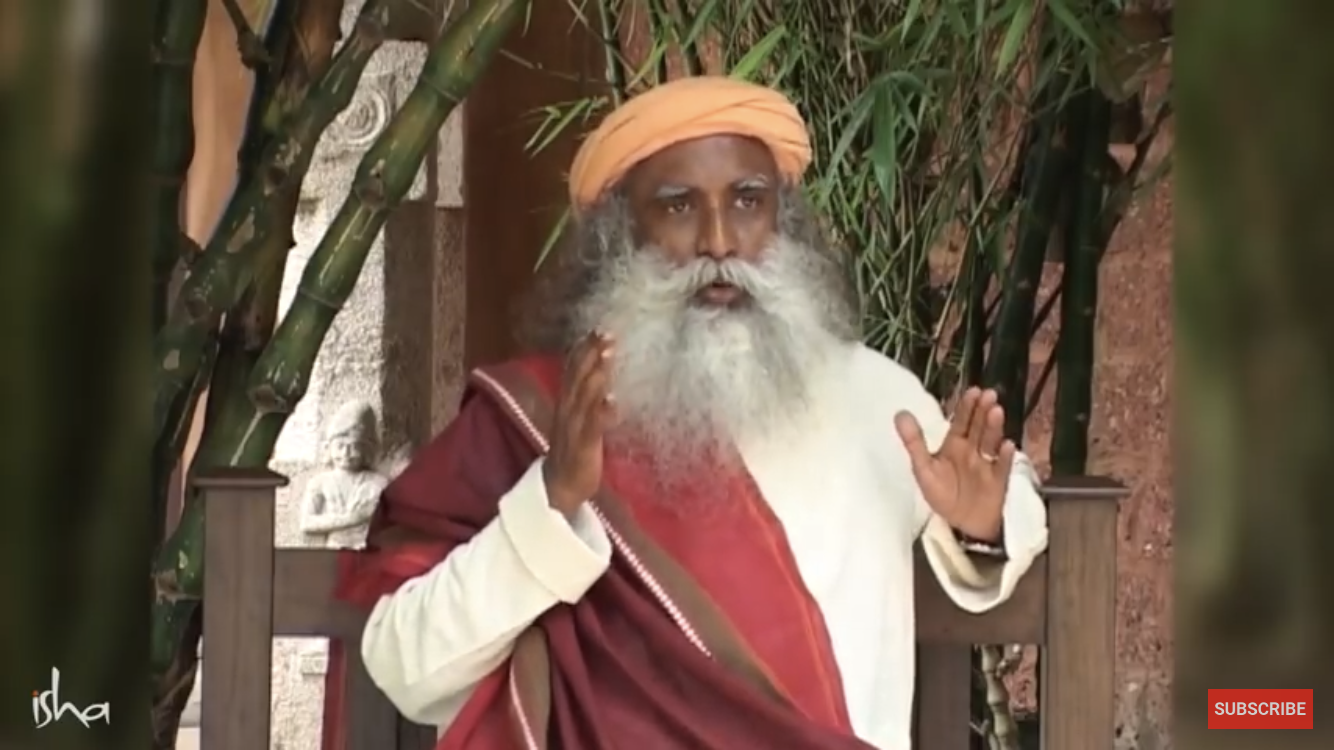
\includegraphics[width=0.5\textwidth]{tooWide} \end{center}

\item Устаревшие заставки <<Sadhguru. Yogi, mystic and visioner.>> и <<Conversation with Mystic>> вырезаются. {\color{gray}Они только отнимает время.}

\item Конечный слайд нужно заменять на \href{https://drive.google.com/file/d/11NbSgvq8LbxDcy-a2WY5OJTKUZKcZx88/view?usp=sharing}{русский}. 

	Конечная надпись <<\textcopyright\ Sadhguru 2021>> не меняется.

 Часто используемые слайды на 
\href{https://drive.google.com/drive/folders/1O54z3DtKpl90ut0Aa8wYkEEP37e00zPY?usp=sharing}{Google Drive}.

\item Вставки с текстом (например, вопросов). Если текст не озвучивается, то время фрагмента с текстом должно быть достаточным, чтобы вы могли неспеша прочитать его (возможно, придется удлиннить видео).

\item Английский текст при переводе не должен быть виден. В случае сложной анимации, этим можно пренебречь в угоду общей эстетики.

\item Любой сколько-нибудь сложный перевод, особенно если есть какие-то названия, нужно согласовать с отвественным человеком (Юрий Кузмин или Ксения Ошерова).

	Перевод вопросов и т.д. обычно имеется у звукоря.

\item Дизайнерский отдел Иши дал следующие шрифты: Merriweather для заголовков, крупного текста и Open Sans для субтитров. Используем их.

    Иногда используется Segoe Script, вы его сразу заметите.

 
\includegraphics[width=0.3\textwidth]{segoeScript}

    Их можно скачать и установить из Google Fonts:
    \begin{itemize}
        \item  Merriweather \href{https://fonts.google.com/specimen/Merriweather}{\small https://fonts.google.com/specimen/Merriweather};
        \item Open Sans \href{https://fonts.google.com/specimen/Open+Sans}{\small https://fonts.google.com/specimen/Open+Sans};
    \item Segoe Script \href{https://www.fonts.com/font/microsoft-corporation/segoe-script?QueryFontType=Web&src=GoogleWebFonts}{\small https://www.fonts.com/font/microsoft-corporation/segoe-script?QueryFontType=Web\&src=GoogleWebFonts}.
      \end{itemize}


\item Переходы между фрагментами с разным фоном через Dip to Black, иначе через Dissolve.

\item Текст без особого смысла, вроде "Darshan — Dec 2012
   Isha Yoga Center" оставляем как есть, наше время ценнее =).
\end{enumerate}

\subsection{Советы}
\begin{enumerate}

\item Для пользователей MacOS самый простой вариант монтирующей системы~--- iMovie, но у нее есть три серьезных недостатка.
    \begin{itemize}
    \item Нет возможности добавить текст поверх видео. То есть, придется делать картинку с перевдодм в отдельном приложении и наклеивать поверх. Это нарушает поток, и геморно исправлять текст.
    \item Можно использовать только два видео трека. Это ограничивает более сложных монтаж, хотя обычно двух хватает.
    \item Нет возможности почеловечески кастомизировать разрешение и формат видео. 
\end{itemize}
Поэтому совет~--- скачать более профессиональное приложение. В ашраме в основном используется Adobe Premiere Pro, насколько я слышал. 

Чтобы его спиратить, наберите в Youtube "Premiere Pro download MacOS free" и выберите видео с большим числом просмотров и положительными отзывами.
\end{enumerate}



\subsection{Тренировочное видео}
\href{https://www.youtube.com/watch?v=9sGJUR7stzc}{Оригинал.}
\quad
\href{https://drive.google.com/file/d/1Y6ECjMSvkaUFmNawIePfFvqS2ZnB3SPi/view?usp=sharing}{Аудио трек.}
\quad
\href{https://www.youtube.com/watch?v=Q3NYDF4JyTg}{Русскоязыное видео для сравнения.}

Название видео: \textbf{Как прожить невероятную жизнь}
	
Перевод субтитра на 08:10: \textbf{Тайир на тамильском означает йогурт}


\begin{wrapfigure}{r}{0.3\textwidth}
  \begin{center}
    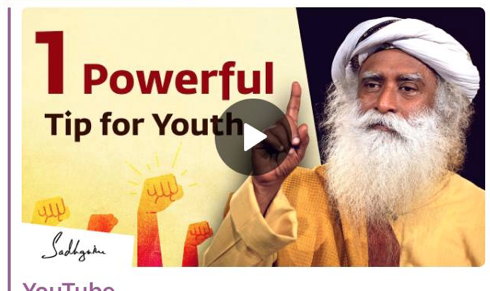
\includegraphics[width=0.28\textwidth]{thumbnail}
  \end{center}
\end{wrapfigure}
PS: Справа~--- thumbnail. Его делает команда дизайнеров, не монтажер.

Хотя, если интересно делать — напишите Юре.



\tikz[remember picture,overlay] \node[opacity=0.15,inner sep=0pt] at (current page.center){
\includegraphics[width=0.2\paperwidth]{IshaLogo}};
\end{document}
% https://www.youtube.com/watch?v=4UH7lzptFH8
